\documentclass[12pt,fleqn]{scrreprt}

\usepackage[ngerman]{babel}
\usepackage[top=2.5cm,bottom=2.5cm,left=2.5cm,right=2.5cm]{geometry}
\usepackage[utf8]{inputenc}
\usepackage{paperandpencil}
  

\usepackage{float}
% Grafik
\usepackage[pdftex]{graphicx}
\begin{document}


\section*{Einverständniserklärung zum Test}
\line
TestNr.: \rule{1cm}{.1pt} \\
\vspace{1cm}

\subsection*{Dank und Information}
Vielen Dank, dass Sie sich die Zeit nehmen und an diesem Test teilnehmen. 
Vor Beginn des eigentlichen Tests erhalten Sie einen kurzen Fragebogen zu Ihrer Person. 
Im Anschluss wird Ihnen das Aufzeichnungsgerät aufgesetzt. 
Bitte beachten Sie, dass die Elektroden mit Kontaktlinsenflüssigkeit befeuchtet sind, 
sollten Sie allergisch auf Kontaktlinsenflüssigkeit sein, dann teilen Sie uns dies bitte mit.
Nachdem die Signalerfassung im grünen Bereich ist beginnt die Kalibrierung des Aufzeichnungsgeräts.
Der eigentliche Test ist in drei Testabschnitte unterteilt.
Bei  jedem dieser Abschnitte soll ein kleiner Fragebogen ausgefüllt werden.
Im Verlauf des Tests werden physiologischen Daten (EEG) aufgezeichnet und gespeichert. 
Die Aufnahmen werden absolut vertraulich und anonym behandelt und nicht an Dritte weitergegeben. 
Die erhobenen Daten werden ausschließlich für die Forschung verwendet und können in diesem Sinne in anonymisierter Form veröffentlicht werden. 
Bitte lesen Sie die unten stehende Einverständniserklärung und unterschreiben Sie an der dafür vorgesehenen Stelle.
Nochmals vielen Dank.\\


\vspace{2cm}
\subsection*{Einverständniserklärung}
Ich weiß, dass physiologischen Daten aufgezeichnet werden. Ich gebe die Erlaubnis, diese erhobenen Daten in anonymisierter Form, für Veröffentlichungen und zur Weiterverarbeitung zu wissenschaftlichen Zwecken, zu verwenden.



\vspace{2.5cm}

\begin{minipage}[b]{0.45\textwidth}	
\line\\
 Ort, Datum
\end{minipage}
\hspace{2cm}
\quad
\begin{minipage}[b]{0.45\textwidth}
\line \\
 Unterschrift
\end{minipage}


\pagebreak
\section*{Erklärung des Tests}
\line
TestNr.: \rule{1cm}{.1pt} \\
\vspace{1cm}

Auf dem Bildschirm werden Sie gleich das unten stehende Bild sehen.
Dabei handelt es sich um die Matrix einen sogenannten "`Spellers".
Ihre Aufgabe wird es sein, mit Hilfe des Spellers zunächst das Wort "`BRAIN"' und dann das Wort "`ISLAND"' zu schreiben.
Diese beiden Worte werden im gesamten Verlauf insgesamt je drei mal zu schreiben sein.\\

\begin{figure}[h!]
\begin{center}
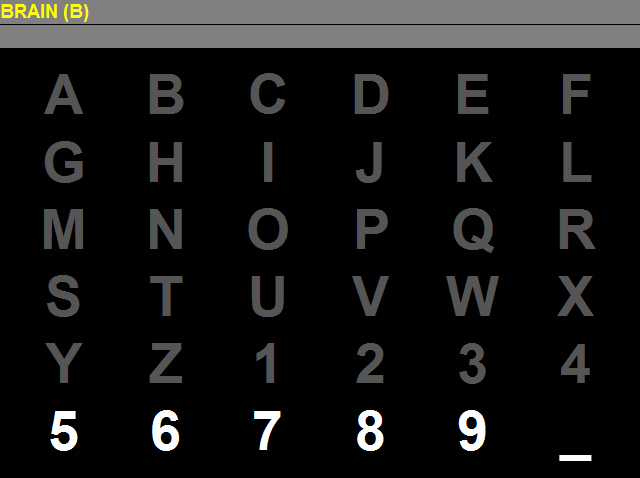
\includegraphics[scale=0.6]{images/speller.png}
%\caption{Die Matrix des Spellers mit aufleuchtender Zeile}
\label{speller}
\end{center}
\end{figure}

Für die Ermittlung Ihres Buchstaben wird der Speller in einer zufälligen Sequenz die Zeilen und Spalten einzeln aufleuchten lassen.
Sie müssen sich in dieser Zeit auf den Buchstaben konzentrieren.
Hilfreich ist es leise in Gedanken zu zählen, wie oft der gewünschte Buchstabe dabei aufleuchtet.
Zwischen jeder Sequenz ist immer eine kurze Pause von 2 Sekunden, danach beginnt eine neue Sequenz, um einen weiteren Buchstaben zu ermitteln.
Bitte vermeiden Sie während der Sequenz zu blinzeln oder sich anderweitig zu bewegen. 
Blinzeln Sie bitte möglichst immer nur in den Pausen zwischen einer Sequenz.
Die Ergebnisse können anderenfalls verfälscht werden.\\





\pagebreak
\section*{Erklärung des Test-Spiels}
\line
TestNr.: \rule{1cm}{.1pt} \\
\vspace{1cm}

In diesem Testabschnitt wird das Konzept des Spellers auf ein Spiel angewendet, 
das Sie in den beiden Abbildungen unten sehen können.


\begin{figure}[ht]
\centering
\begin{minipage}[b]{0.46\linewidth}	
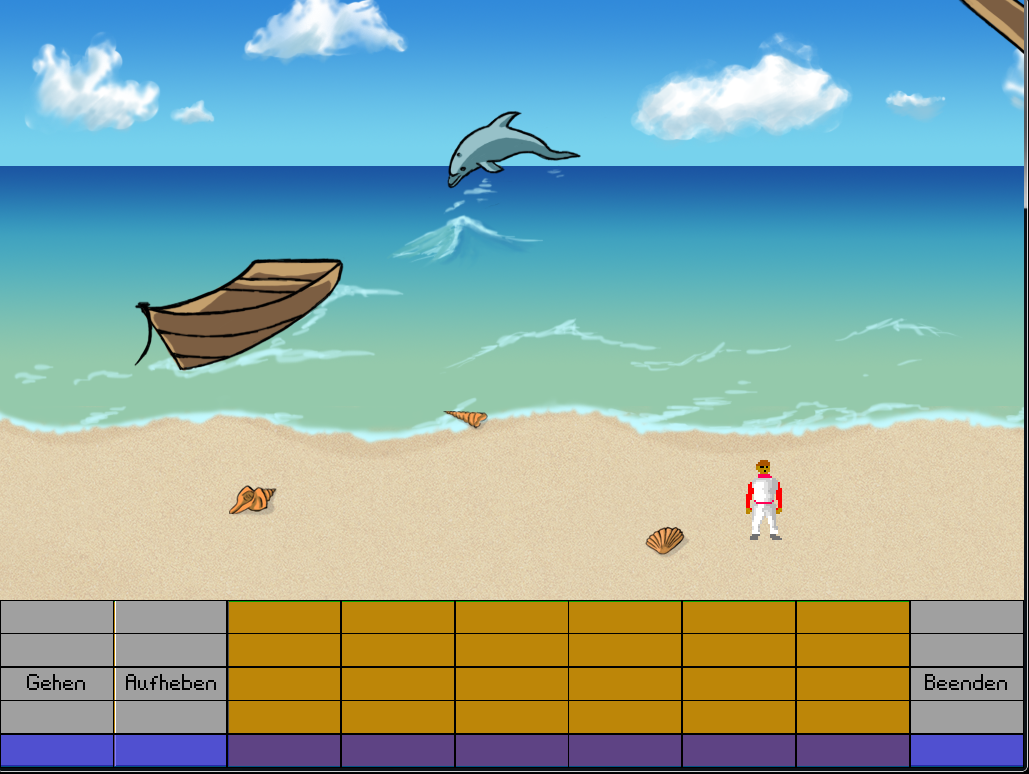
\includegraphics[scale=0.28]{images/befehlsmatrix.png}
%\caption{Die Matrix zur Auswahl eines Befehls für die Spielfigur}
\label{control}
\end{minipage}
\quad
\begin{minipage}[b]{0.46\linewidth}
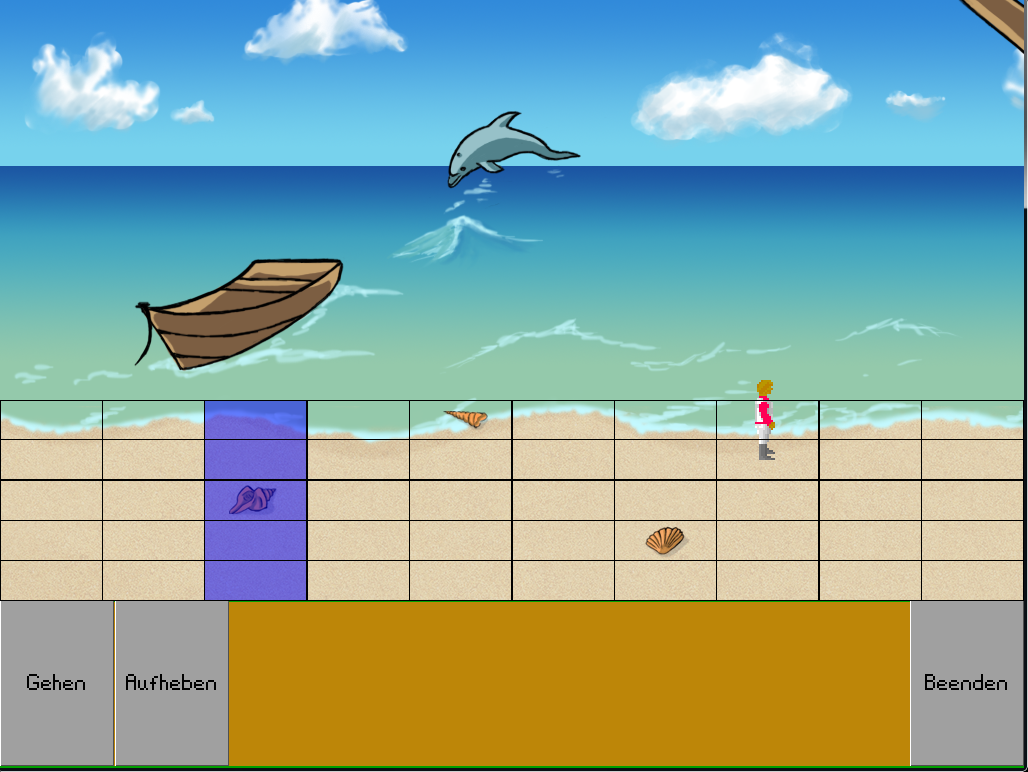
\includegraphics[scale=0.28]{images/strandmatrix.png}
%\caption{Die Auswahl eines Ziels für einen Befehl}
\label{target}
\end{minipage}
\end{figure}


In diesem Spiel müssen Sie nun statt der Buchstaben bestimmte Felder auswählen.

Ihre Aufgabe innerhalb des Spiels ist es:
\begin{itemize}
\item alle Objekte auf dem Strand von links nach rechts aufzuheben
\item an den rechten Rand des Strandes zu laufen, um die Szene zu einem weiteren Strand\-abschnitt zu wechseln
\item ebenfalls alle Objekte dieses Strandabschnitts aufzuheben
\end{itemize}

Das Spiel wird beendet, sobald Sie alle Objekte aufgehoben haben oder Sie 25 Eingabe-Ermittlungen durchgeführt haben.\\

Benutzen Sie dazu bitte diese beiden Befehle:\\

\begin{minipage}[b]{0.13\linewidth}	
\textbf{Aufheben}: \\ \\ \\ \\ 
Wichtig!\\

\end{minipage}
\quad
\begin{minipage}[b]{0.79\linewidth}
Wählen Sie diesen Befehl und anschließend ein Zielfeld mit einem Objekt, damit die Spielfigur sich dorthin bewegt und den Gegenstand aufhebt.
Falls Sie ein freies Feld auswählen, wird die Figur stehen bleiben und sagen, dass es dort nichts zum Aufheben gibt.\\
Konzentrieren Sie sich für diesen Befehl auf das Feld, in dem "`Aufheben"' steht.
\end{minipage}

\vspace{1.25cm}

\begin{minipage}[b]{0.13\linewidth}	
\textbf{Gehen}: \\ \\ 
Wichtig! \\

\end{minipage}
\quad
\begin{minipage}[b]{0.79\linewidth}
Mit diesem Befehl können Sie an eine Position auf dem Strand laufen, um so an den rechten Rand des Strandes zu gelangen.\\
Konzentrieren Sie sich für diesen Befehl auf das Feld, in dem "`Gehen"' steht.
\end{minipage}












\pagebreak
\section*{Fragen zur Person} 
\line
TestNr.: \rule{1cm}{.1pt} \\



\begin{minipage}[b]{0.45\textwidth}	
\question*{\textbf{Geschlecht?}}
\begin{longanswersB}
\item weiblich
\item männlich
\end{longanswersB}
\end{minipage}

\vspace{0.75cm}

\begin{minipage}[b]{0.45\textwidth}	
\question*{\textbf{Sind Sie Brillenträger?}}
\begin{longanswersB}
\item Ja
\item Nein
\end{longanswersB}
\end{minipage}
\hspace{2cm}
\quad
\begin{minipage}[b]{0.45\textwidth}
\question*{\textbf{Tragen Sie Kontaktlinsen?}}
\begin{longanswersB}
\item Ja
\item Nein
\end{longanswersB}
\end{minipage}


\question*{\textbf{Sind bei Ihnen neurologische oder mentale Erkrankungen bekannt?}}
\begin{longanswersB}
\item Ja, welche \rule{10cm}{.1pt}%
\item Nein
\end{longanswersB}


\question*{\textbf{Stehen Sie unter dem Einfluss von Medikamenten/Drogen/Alkohol?}}
\begin{longanswersB}
\item Ja, welche \rule{10cm}{.1pt}%
\item Nein
\end{longanswersB}

\question*{\textbf{Haben Sie vor kurzem übermäßig viel koffeinhaltige Produkte konsumiert? }}
\begin{longanswersB}
\item Ja
\item Nein
\end{longanswersB}

\question*{\textbf{Haben Sie bereits Erfahrung/Übung mit Brain Computer Interfaces? }}
\begin{longanswersB}
\item Ja
\item Nein
\end{longanswersB}


\vspace{0.75cm}
\line \\


\pagebreak
\section*{Fragebogen Testabschnitt 0 }
\line
TestNr.: \rule{1cm}{.1pt} \\



Bitte stufen Sie bei den nachfolgenden Fragen ihre Antworten innerhalb der Skala von 1 bis 10 ein.
Beachten Sie inbesondere die beistehende Beschriftung der jeweiligen Skalenwerte.

\question*{{\textbf{Wie müde fühlen Sie sich im Moment?}}}
\hupBten{{\textbf{nicht müde}}}{ {\textbf{sehr müde}}}

\question*{{\textbf{Wie fühlen Sie sich allgemein?}}}
\hupBten{{\textbf{nicht gut}}}{ {\textbf{sehr gut}}}
Anmerkungen? \rule{10cm}{.1pt}%




% Test 1 = Nach dem Vorher-Test 
% Test 2 = Nach dem Test-Spiel
% Test 3 = Nach dem Nachher-Test









\pagebreak
\section*{Fragebogen Testabschnitt 1 }
\line
TestNr.: \rule{1cm}{.1pt} \\

Bitte stufen Sie bei den nachfolgenden Fragen ihre Antworten innerhalb der Skala von 1 bis 10 ein.
Beachten Sie inbesondere die beistehende Beschriftung der jeweiligen Skalenwerte.


\question*{{\textbf{Wie müde fühlen Sie sich im Moment?}}}
\hupBten{{\textbf{nicht müde}}}{ {\textbf{sehr müde}}}

\question*{{\textbf{Wie fühlen Sie sich allgemein?}}}
\hupBten{{\textbf{nicht gut}}}{ {\textbf{sehr gut}}}
Anmerkungen? \rule{10cm}{.1pt}%

\question*{{\textbf{Wie schwer fiel es Ihnen sich auf die Matrix-Elemente zu konzentrieren?}}}
\hupBten{{\textbf{nicht schwer}}}{ {\textbf{sehr schwer}}}











\pagebreak
\section*{Fragebogen Testabschnitt 2}
\line
TestNr.: \rule{1cm}{.1pt} \\

Bitte stufen Sie bei den nachfolgenden Fragen ihre Antworten innerhalb der Skala von 1 bis 10 ein.
Beachten Sie inbesondere die beistehende Beschriftung der jeweiligen Skalenwerte.

\question*{{\textbf{Wie müde fühlen Sie sich im Moment?}}}
\hupBten{{\textbf{nicht müde}}}{ {\textbf{sehr müde}}}

\question*{{\textbf{Wie fühlen Sie sich allgemein?}}}
\hupBten{{\textbf{nicht gut}}}{ {\textbf{sehr gut}}}
Anmerkungen? \rule{10cm}{.1pt}%

\question*{{\textbf{Wie schwer fiel es Ihnen sich auf die Matrix-Elemente zu konzentrieren?}}}
\hupBten{{\textbf{nicht schwer}}}{ {\textbf{sehr schwer}}}









\pagebreak
\section*{Fragebogen Testabschnitt 3}
\line
TestNr.: \rule{1cm}{.1pt} \\

Bitte stufen Sie bei den nachfolgenden Fragen ihre Antworten innerhalb der Skala von 1 bis 10 ein.
Beachten Sie inbesondere die beistehende Beschriftung der jeweiligen Skalenwerte.


\question*{{\textbf{Wie müde fühlen Sie sich im Moment?}}}
\hupBten{{\textbf{nicht müde}}}{ {\textbf{sehr müde}}}

\question*{{\textbf{Wie fühlen Sie sich allgemein?}}}
\hupBten{{\textbf{nicht gut}}}{ {\textbf{sehr gut}}}
Anmerkungen? \rule{10cm}{.1pt}%

\question*{{\textbf{Wie schwer fiel es Ihnen sich auf die Matrix-Elemente zu konzentrieren?}}}
\hupBten{{\textbf{nicht schwer}}}{ {\textbf{sehr schwer}}}


\question*{\textbf{Möchten Sie uns etwas in Bezug auf die Tests mitteilen?}}
\openthree








\end{document}